\documentclass{UoYCSproject}
\usepackage{booktabs}
\addbibresource{dummyBib.bib}
\author{Lilian Blot}
\title{An example of a project reports in \LaTeXe\ with the   \textsf{UoYCSproject} class}
\date{Version 3.0, 2020-November}
\supervisor{Jeremy L. Jacob}
\BSc
 \usepackage{rotating}
 \usepackage{tabularray}
 \usepackage{rotating}
 \usepackage{tabularray}
 \dedication{To all students everywhere}
 \usepackage{graphicx}


\acknowledgements{
  I would like to thank my goldfish for all the help it gave me
  writing this document.

  As usual, my boss was an inspiring source of sagacious advice.
}

% More definitions & declarations in example.ldf
\begin{document}
\pagenumbering{roman}
\maketitle
\listoffigures
\listoftables
%\usepackage{booktabs}

%\renewcommand*{\lstlistlistingname}{List of Listings}
%\lstlistoflistings


    \chapter{Introduction}
    \label{ch:introduction}
    \setcounter{page}{1}
    \pagenumbering{arabic}

    Introduction
    Late delivery of software projects remains an ever present challenge, often attributed to the inherent uncertainties and complexities associated with development.
    There are multiple factors that affect the delivery of a software project, however it is clear that project planning plays a role in this. \cite{CHOW2008961}. \par
    Agile Software development is a type of iterative planning method where a project is broken up into smaller “user stories” or tickets, each defining a specific task or part of a project that must be completed.
    Generally each ticket has an estimate attached to it, defining the time or effort it will take to finish.
    Some projects use time-based estimates like hours or days to estimate tickets, others teams assign “Story Points”, an abstract unit of perceived complexity, risk, and effort involved in implementing a specific feature or piece of functionality.
    For example, a Story Point value of 1, may be equated to 2 hours work or less, 8 around 22 hours of active work on a ticket or 11 hours for 2 people.
    It is common for the Story Point scale used to be an adjusted fibbonaci, of 1, 2, 3, 5, 8, 13, 15, 20, 40, 100.
    Estimates enable a Team leader to plan what tickets can be completed in a “sprint”, or “iteration”, usually a period of 2-4 weeks, based on how many points they think the team will be able to do.
    The number of story points that a team is able to complete in a single iteration is known as the teams "Velocity" \cite{cohn2005agile}.
    The process for estimating tickets can be time consuming, the faster that a ticket is estimated, the faster it can be planned for completion.
    Furthermore, the more accurate an estimation is, the more likely it is that a release, which in agile, is a collection of tickets associated with features or bug-fixes in a release, can be delivered on time, as the work will have been planned accordingly. \par

    When a ticket is created, it is placed into a to-do list of tickets called a “backlog”.
    Tickets in the backlog are then estimated for their effort or time to complete, and are then ordered according to multiple factors including this estimate and the priority of the ticket.
    Generally in projects, work cannot be carried out on a ticket until it has been estimated.
    This emphasises the importance of both the speed and accuracy of ticket estimation in the successful management of projects.
    Automated ticket estimation may enable the correct prioritisation of tickets before any estimation activities are carried out by the team or members of the team.
    By using a large language model, the information provided in a tickets title and description can be used as features in a classification neural network.
    The model proposed in this paper is intended to participate in the estimation process rather than perform the estimation as the source of truth.
    This is because incorrect estimates can have severe consequences on project planning, a model would need to be extremely accurate in order to be trusted to estimate the ticket correctly.
    In practice the model participation can happen in multiple ways.
    The model may act as an advisor for the “expert” who is estimating tickets.
    Alternatively the model may participate in agile poker sessions with members of a project, whereby engineers play a “game” where everyone chooses a card that equates to the value that they want to estimate, then discuss and re-estimate until a consensus is reached \cite{1667560}. \par

    In order to simplify the problem, the model proposed in this paper will be able to classify tickets into 3 categories, “Small”, “Medium” and “Large”.
    When inspecting data from a project in a large automotive company, who estimate using minutes and hours, it was found that the accuracy of ticket estimation was 74\% when using the above categories.
    Therefore the model proposed in this paper will aim to achieve an accuracy of 70\% or higher in order to be useful.
    Furthermore, I am aiming to ensure that the model takes less than 4 hours to train, and less than 1 second to classify a ticket once trained.
    This is so that the model can be used in real time, and can be retrained on a regular basis to ensure that it is up to date with the latest data, ensuring continuous learning but also reduce costs. \par


    \chapter{Literature Review}
    \label{ch:literature-review}
    This section discusses the current research into methods of ticket estimation, including with Deep learning, as well as in the broader field of Natural Language Processing.
    It summarises and analyses existing work as well as highlighting unknowns within the topics.

    It is broken down into 3 sub-sections.
    First “Estimation in Software Engineering Projects” focuses on research about effort and time estimation as a concept, as well as research into techniques for doing estimations.
    The next sub-section focuses on relevant research into Large Language Models and Natural Language Processing.
    Lastly, the “Agile Estimation with Deep Learning” looks at Deep learning models specifically for classification of text, particularly of Agile Tickets for estimation.


    \section{Effort Estimation}
    \label{sec:effort-estimation}
    Current research into estimation in agile projects mostly centres around how estimations are produced and what scale they use.
    There are many methods for estimating tickets or projects that have been examined in academic research.
    They can be sorted into two main categories, Judgement-based approaches and Model-based approaches (discussed below).

    \subsection{Judgement-based approaches}
    \label{subsec:judgement-based-approaches}

    Judgement-based approaches rely on the knowledge of experts about the field or project in question, who can make an estimate based on their experiences and knowledge on how much effort a ticket will take to complete.
    The simplest judgement based approach, expert judgement, is a single expert estimating the ticket by themselves, however group estimation techniques such as Planning poker, whereby team members play a “game” to reach an agreement on the Story Point estimate of a tickets are also popular.
    Research has been done to examine the accuracy of these techniques by looking at the result of the same ticket estimated with both, showing that planning poker is more accurate that individual expert estimates \cite{MAHNIC20122086, RashidSCE}. Other
    In 2015, a survey was performed to determine the state of the practice of Effort Estimation of Agile Software Development, claiming to be the first of its kind.
    The research surveyed 60 users of agile practices across 16 different countries. It established that 63\% of participants use Planning poker to perform estimations followed by 47\% used Analogous estimating (whereby parallels are drawn from previous stories and they are used to decide an estimate for new stories) and expert judgment (38\%) \cite{0.1145/2745802.2745813}.

    \subsection{Model-based approaches}\label{subsec:model-based-approaches}
    In the last 30 years, many Algorithmic-Based Approaches have been proposed to automate the estimation of tickets
    and projects.
    In 1981, the Constructive Cost Estimation Model ($COCOMO$) model was proposed by DR. Berry Boehm \cite{Boehm2001}.
    The basic $COCOMO$ model defines the effort required to complete a project to be $a^2 \times (KLOC)a^2pm$.
    Where $KLOC$ is kilo lines of code, $a$ is a constant depending on the type of project and is expressed in person months ($pm$), the detailed version adds effort multipliers for each phase of a project, splits the effort estimation into subsystems and adds various extra multipliers to improve accuracy.
    Although this model can achieve a mean average accuracy of 91\% for effort estimation on projects, the model requires a lot of input information, including Lines of Code, number of files, number of external interfaces and developer experience with the technical stack.
    COCOMO, as well as other model based estimators and regression models, are used much less in agile software development than previously in non-agile development methods due to the estimations being for tickets rather than for entire projects, where the attributes needed are more readily available and relevant and the planning stages are more extensive \cite{10.1145/2745802.2745813}.
    As in a ticket rather than in a project, the main information is the textual description, with the shift towards agile software development, focus has shifted towards researching how we can leverage Natural Language Processing in order to estimate story points.


    \section{Large Language Models}
    \label{sec:large-language-models}
    Large Language Models (LLM) are a type of artificial intelligence model that is designed to understand, generate
    or manipulate human language.
    These models are characterized by their size and complexity, often consisting of millions or even billions of parameters.
    Large language models are built on advanced deep learning architectures and are typically pre-trained on massive amounts of textual data (corpus) before being fine-tuned for specific tasks. \par

    In 2017, transformer based architecture was introduced in a model proposed by Vaswani et al. in their paper, "Attention is all you need" \cite{vaswani2023attention}.
    It has become the foundational model for a variety of natural language processing (NLP) tasks, including text classification, question answering, summarization, and translation.
    The transformer based architecture is a type of neural network architecture that is designed to process sequential data, such as text, and is based on the concept of attention.
    The core innovation of this architecture is the introduction of 'self-attention'.
    Self-attention allows a model to weigh the importance of different words in a sequence when processing each word, rather than relying on a fixed-length context window, like in recurrent neural networks (RNNs).
    It also allows the model to process all words in a sequence simultaneously, rather than sequentially, therefore improving the training speed as it allows parallelization.
    The mechanism computes attention scores for each token in the input sequence, indicating how much attention should be paid to other tokens.
    By considering relationships between all tokens simultaneously, the model can capture long-range dependencies and contextual information effectively.
    To capture diverse types of information and relationships, the self-attention mechanism is typically divided into multiple attention "heads".
    Each head independently computes attention scores, allowing the model to focus on different aspects of the input.
    By combining information from multiple heads, the model can capture a richer set of features and relationships within the sequence.
    \par
    In June 2018, Generative Pre-Trained Transformers (GPT) was introduced by OpenAI in the paper "Improving Language Understanding by Generative Pre-Training".
    GPT follows an autoregressive approach during both pre-training and fine-tuning, this means that the model generates text sequentially, predicting the next word in a sequence based on the preceding context.
    This allows GPT to capture complex dependencies and relationships in language, however GPT only looks at the context of previous words, left-to-right rather than bidirectionally like later models.

    In October 2018, the Bidirectional Encoder Representations from Transformers (BERT) model was introduced by Devlin et al \cite{devlin2019bert} .
    BERT is a large language model that uses the transformer architecture and is pre-trained on a large corpus of unlabelled text, including the entire Wikipedia corpus and a large book corpus, totaling 3,300M words.
    It is trained using a masked language model (MLM) objective, where random tokens in a sequence are masked, and the model is trained to predict those masked tokens.
    BERT is considered a landmark in the development of large language models, for multiple reasons.
    An important difference between BERT and previous language models is that it is bidirectional, meaning that it can
    use the context of both the left and right side of a word when processing it, enabling the model to capture richer contextual information compared to previous unidirectional models.
    At time of release, BERT outperformed all other Large Language Models on the General Language Understanding Evaluation (GLUE Benchmark), a set of tasks that are designed to measure the performance of models that aim to understand language.
    An average of 79.6\% on the $GLUE$ benchmark tasks was achieved by the $BERT_{base}$, 4.4\% higher than the previous highest score achieved by OpenAI's GPT.

    The release of BERT and GPT in 2018 was followed by the proposal of many new models based on the transformer architecture in 2019.
    XLNet was introduced by researchers at Google and Carnegie Mellon University, it is another transformer-based language model that extends the bidirectional context understanding of BERT while addressing some of its limitations.
    XLNet uses a permutation language model (PLM) objective.
    Instead of masking random tokens, XLNet considers all tokens in the sequence as potential candidates for prediction.
    This means that the model is trained to predict the probability distribution over all possible permutations of the sequence.


% This part is maybe not neccessary?
%    An important part of Large language models is Tokenization, which is the process of splitting a string into a list of
%    tokens.
%    A token can be a word, sentence, paragraph or even a single character.
%    Tokenization is performed by a Tokenizer, which is a class that defines a vocabulary and methods for encoding.
%    The vocabulary is a list of known tokens, for example words from a dictionary or in a particular corpus.
%    The Tokenizer can then encode a string by breaking it up into tokens and replacing each token with its corresponding integer value from the vocabulary.
%    One popular tokenizer is WordPiece, which was introduced in 2016 by Google as the tokenization method for BERT [BERT].
%    WordPiece is a sub-word tokenizer, meaning that it breaks words down into smaller parts, or sub-words.
%    It is effective in handling rare or unseen words because it can represent them as a combination of more common sub-word units.
%    This property is especially valuable for tokenizing text on a niche topic or with unusual vocabulary. \par
%
%    Byte Pair Encoding (BPE) is another popular tokenizer, it was first introduced by Philip Gage in the context of text compression in 1994 [BPE].
%    It is a simple form of dictionary encoding, which iteratively replaces the most frequent pair of bytes in a sequence with a single, unused byte.
%    Whilst it was an effective text compression algorithm, it was later recognized for its utility in natural language processing (NLP),
%    and has since been used in many NLP models, including transformer-based models like GPT.


    \section{Ticket classification with deep learning}
    \label{sec:estimation-with-deep-learning}

    In 2018, Choetkiertikul et al.
    introduced a significant contribution to the field of software engineering with their paper titled 'A deep learning model for estimating story points.' \cite{8255666}.
    This research, conducted at the University of Wollongong (Australia), presents a model for estimating the story point estimation of tickets (DEEP-SE) and is the most notable research paper on ticket classification with deep learning.
    The model uses long short-term memory and recurrent highway network which are both types of recurrent neural network (RNN) architectures.
    It defines the task as a regression problem and achieves a standardized accuracy of 52.66\%
    \[SA = (1-\frac{MAE}{MAE_{rguess}}) \times 100\]
    where $MAE$ is the Mean Absolute Error and $MAE_{rguess}$ is the MAE of a large number (e.g. 1000 runs) of random guesses. Such that $MAE$, defined as \[ MAE = \frac{1}{N}\sum_{i=1}^{N}|ActualSP_{i} - EstimatedSP_{i}|\] where $N$ is the number of issues used for evaluating the performance (i.e. test set), $ActualSP_i$ is the actual story point, and $EstimatedSP_i$ is the estimated story point, for the issue $i$.
    The dataset used for this model was 23,313 tickets story points, collected from 16 large open source projects.
    This dataset has since been used by other researchers including Phan et al\. who looked at the potential and possible challenges of Graph Neural Network text
    classification in story point estimation \cite{phan2022story}.
    The proposed model from Choetkiertikul et al. achieved an accuracy as high as 80\% on some projects within the dataset when classifying tickets into 6 'buckets' of story points.
    Despite the model performing well, the validity of the model is in question, as the data that the model was trained on was from open source projects, and although the paper claims the story points in the dataset are accurate, it is not clear how this was verified.

    It is clear that there is a research gap into ticket effort estimation using large language models such as BERT.
    The model proposed in this paper aims to contribute towards filling this gap by using a large language model to classify tickets into 3 categories, “Small”, “Medium” and “Large”.

    \chapter{Ethical Considerations}
    As with any machine learning model, there are ethical considerations to be made.

    The BERT models are known to have biases, particularly in relation to race and gender due to the corpus of text it was trained on.
    These biases are hard to remove, and are a topic of ongoing research in the field of machine learning. Particularly in relation to Gender Bias \cite{Jentzsch_2022, li2021detecting}.
    To mitigate the risk of bias, I have removed all names. Although it is rare for pronouns to be used in tickets, I also removed the few references to gendered pronouns that were present.
    This is to ensure that the model does not learn to associate the prediction with a particular person or gender.

    The model is not intended to replace the estimation of tickets, but to assist in the process. This is because the model is not 100\% accurate, and incorrect estimates can have severe consequences on project planning.
    It would not be ethical to use the model to estimate tickets without human oversight. Particularly as the estimation of tickets can be used to examine the performance of team members, and therefore affect their career progression.

    I have not sought approval from the ethics committee as the topic of the project is not sensitive, and the data has been anonymized.

    Permission has been sought from the company to use the data, and the data has not been made public to ensure that no sensitive information is leaked.


    \chapter{Methodoloy}
    \label{ch:methodology}
    This section introduces the proposed model for the classification of software development tickets.
    It covers explanation of the datasets, preprocessing, data augmentation methods and the architecture of different transformer models that were evaluated as layers in the final model.
    The last subsection discusses the ethics of the problem.


    \section{Datasets}\label{sec:datasets}
    The datasets used to evaluate this model come from a large automotive software company, containing a total of 19,500 tickets, across 7 projects.
    An example ticket is shown in figure \ref{fig:ticket}.
    Every ticket has a title, or a "Summary" that is a short description of the ticket which usually less than X words. This is shown in box A of the figure.
    It then has a description, this a longer piece of text that explains what the aim of the ticket is as well as additional information such as design decisions, criteria for the ticket and links to related documentation. (Shown in box B) \par

    \begin{figure}[h]
        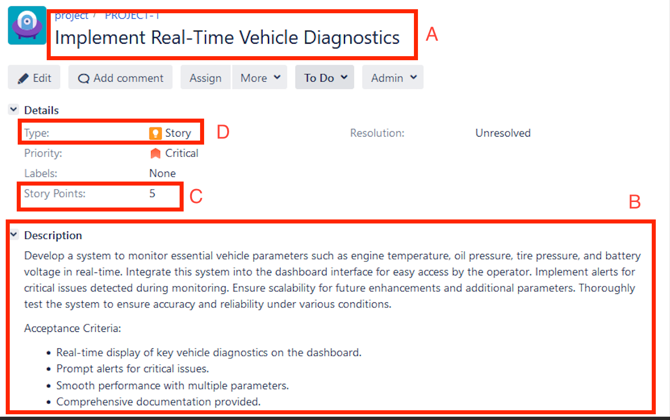
\includegraphics[width=\textwidth]{./figures/dummy-ticket}
        \caption{an example ticket}
        \label{fig:ticket}
    \end{figure}

    For the dataset in question, the word count in the description is between 2 and 1000, as shown in figure X.

    [TODO: Add graph showing word count of ticket by class, probably a box plot per class]

    The dataset has two types of tickets, ones that have been estimated with a specific time and ones that have been estimated with story points.
    Ones that have been estimated with a specific time also have the "Actual time spent" logged on them.
    This is useful as it may help our model become more 'intelligent' than a person estimating them as we can use true values. \par
    An example story point estimation is shown in figure \ref{fig:ticket}, in box C.
    The projects for this were chosen by looking at projects that have more than 1000 tickets with story points, this is because it is likely that the more tickets that a team has estimated, the more accurate they are at estimating.
    Another requirement was for the tickets to be written only in English, this is because most large language models are language specific.


    \section{Pre-Processing}\label{sec:preprocessing}

    The main features of each ticket is its summary and description.
    The description is written with Jira Markdown syntax, for example it allows formatted blocks of code to be added with the syntax `{code:java} {code}` and `h[1-6].` formats the following text as a heading.
    In order to remove this syntax and reformat the text as plain text, a set of regex replace rules were used.
    These rules removed blocks of code and formatting syntax, but also has anonymised the data by removing mentions of users, for example `@KatieMaison`.
    This stops the model learning to differentiate the estimation for the ticket by a user as a feature, as this may have ethical considerations. \par

    The text string used as an input to the model is the summary prepended to the description.
    This is because usually in a ticket, a title has the most important information in it, often containing keywords about the contents of the ticket. \par
    This is important as the model has a word limit of 512 tokens, and the description is sometimes longer than this, therefore as the description is truncated, the more important information from the summary goes at the start..

    In order to enable classification, an additional column $class$ was added to the dataset, where $class(ticket) \in \{0,1,2\}$, where 0 is small, 1 is medium and 2 is large.
    "Small" tickets have been defined as those that take 1 hour or less to complete and are estimated to be 1 or less Story Point in effort.
    "Medium" tickets have been defined as those that take between 1 and 5 hours, or are estimated to be between 1 and 5 story points.
    "Large" tickets are defined to take more than 5 hours to complete, or have more than 5 story points as an estimate.


%\begin{tabular}{|p{7cm}|p{2cm}|p{1.5cm}|p{1cm}|}
%  \hline
%  Ticket Description & Story Point Estimate & Time Logged & Class\\
%  \hline
%  As part of the AUTOSAR project, we need to implement the Controller Area Network (CAN) communication module. This module will facilitate communication between various electronic control units (ECUs) within the vehicle.
% & 5 & N/A & 1 \\
%    \hline
%
%  Row 2, Col 1 & Row 2, Col 2 & Row 2, Col 3 & c2 \\
%  \hline
%\end{tabular}


    \section{Data Augmentation}\label{sec:data-augmentation}
    In order to increase the generalisation of the model and therefore increase accuracy on unseen data, I have opted to use data augmentation to increase the number of data points.
    Back translation was tested as an augmentation technique, this is where a ticket is translated into a different language, and then translated back.
    I used the NLPAug Python library, which allows you to choose a translation model from huggingface to use to translate the text \cite{ma2019nlpaug}.
    However upon inspecting the tickets, there was very little change in the wording of the ticket, and the model over-fit much more quickly, reaching a very small loss and test accuracy stagnated.
    Instead, paraphrasing had better results.
    To do so, I used a pretrained model from the huggingface library, "Finetuned ChatGPT paraphraser on T5-base". \cite{chatgpt_paraphraser}
    This model is fine-tuned on a dataset of phrases and paraphrases.


    I first used the data cleaner described previously to remove the formatting syntax, then ran the paraphraser on every ticket, generating a single paraphrased version per ticket.
    This took 21 hours on a NVIDIA RTX a4500 Graphics card. An example of paraphrased  \par
    \begin{table}
    \centering
    \begin{tabular}{p{2.5cm}p{9cm}}
    \toprule
    Original    & As part of ensuring compliance with safety regulations, we need to enhance the safety checks within the critical system. This involves reviewing existing safety protocols, identifying potential vulnerabilities, and implementing robust measures to mitigate risks effectively. \\\addlinespace[0.5em]
    Paraphrased & To ensure compliance with safety regulations, we must perform additional safety checks within the critical system. This involves reviewing existing safety protocols, identifying potential vulnerabilities, and implementing robust measures to mitigate risks effectively.       \\
    \bottomrule
    \end{tabular}

    \caption{Example of a paraphrased ticket}
    \end{table}


    \section{Architectures}\label{sec:architectures}
    The architecture of the model can be described in three parts, Tokenization Layer, Transformer Layers and Classification Head.
    These will be described sequentially in the following sections.\par

    [TODO: Add diagram of architecture]\par

    \subsection[tokenization-layer]{Tokenization Layer}
    In order to be used in a Large Language Model, textual input needs to be transformed into tokens and embeddings.
    My model uses the BERT Tokenizer, the specific implementation of which is provided by the transformers huggingface library. \par

    \begin{figure}[h]
        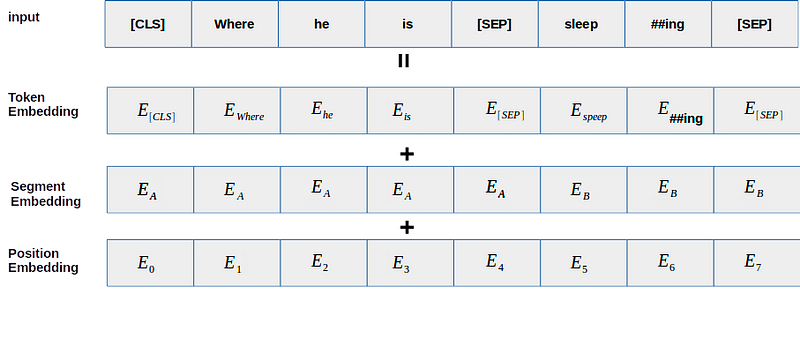
\includegraphics[width=\textwidth]{./figures/bert-tokenizer}
        \caption{Bert Tokenizer from the Original Bert Paper}
        \label{fig:tokenizer-figure}
    \end{figure}

    % Maybe i can add to the tokenizer vocab? https://medium.com/@pierre_guillou/nlp-how-to-add-a-domain-specific-vocabulary-new-tokens-to-a-subword-tokenizer-already-trained-33ab15613a41
    The tokenizer works by splitting each tickets description into individual tokens, then converting these into a numerical value from the models vocabulary, as shown in the example in figure \ref{fig:tokenizer-figure}.
    The tokens are then padded to the length set, in this case 256 and then the tokenized test is passed to the transformer layers.
    The BERT Tokenizer used is uncased, meaning that it turns everything into lower case and removes accents before tokenizing it.
    \par

    One of the benefits of the preprocessing discussed in section \ref{sec:preprocessing} is that it reduces the size of the textual description in the dataset, as it removes a lot of characters.
    This enables the model to get more information from the text, as the model has a word limit of 256 tokens. As each non-alphanumeric character is a token in iteself, this means that the model can get more information from the words in the text once these are removed.
    I tokenized the data before and after preprocessing, and found that the average number of tokens in the description was reduced from 111 to 91, but more importantly, the upper quartile value and upper range was reduced to fall inside of the 256 token limit.
    This is shown in figure \ref{fig:token-boxplot}.

    \begin{figure}[h]
        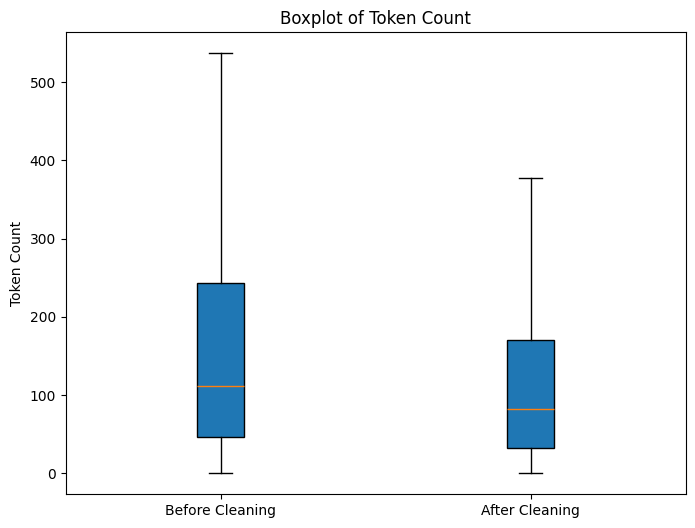
\includegraphics[width=\textwidth]{./figures/tokencount-prepost}
        \caption{Boxplot showing statistics on the number of tokens in the description before and after preprocessing.}
        \label{fig:token-boxplot}
    \end{figure}


    \subsection[transformer-layer]{Transformer Layer}
    The transformer layers are the core of the model, they are the part of the model that is responsible for understanding the context of the tokens.
    A transformer layer is a type of neural network architecture that is designed to process sequential data, such as text, and is based on the concept of attention.
    In a transformer layer, the input is passed through multiple layers of attention and feed forward neural networks.
    As previously discussed, the transformer architectures self attention mechanism allows the capturing of long-range dependencies and contextual information.
    After obtaining contextualized representations through self-attention, the outputs are passed through a feed-forward neural network (FFN).
    This network applies linear transformations and non-linear activation functions to capture complex patterns and relationships within the representations.
    The FFN enables the model to distill and refine the contextual information obtained from self-attention, producing richer and more informative representations of the input sequence.
    In this model, I have experimented with multiple pretrained BERT models that use the transformer architecture that have various benefits, including optimization of training time and size. \par
    The pretrained model is then fine-tuned on the dataset, where it learns the specific context of the tickets in the dataset.

    \par

    \textbf{BERT Base Uncased: Bidirectional Encoder Representations from Transformers}

    This model is the original weights for the pre-trained BERT model, with 12 transformer layers, each with 12 attention heads.
    It is downloaded from the huggingface model hub, and is the most widely used BERT model \cite{bert-base-uncased}.
    \par

    \textbf{BERTOverflow: Code and Named Entity Recognition in StackOverflow}
    BERTOverflow is a BERT model that is pre-trained on a large corpus of 152 million sentences from StackOverflow, a question and answer website for programming questions \cite{tabassum2020code}.
    The architecture of this model is the same as the classic BERT model, however the fine-tuning may enable it to have better context understanding of technical terms.
    \par

    \textbf{DistilBERT: a distilled version of BERT: smaller, faster, cheaper and lighter}
    DistilBert is a smaller version of BERT, it has 6 transformer layers, each with 12 attention heads.
    It is trained using knowledge distillation, a process where a smaller model is trained to mimic the outputs of a larger model.
    This is done by training the smaller model to predict the outputs of the larger model, rather than the ground truth.
    This allows the smaller model to learn from the larger model, and therefore be more efficient.
    DistilBERT is 40\% smaller than BERT and is 60\% faster \cite{sanh2020distilbert}.
    \par

    \textbf{ALBERT: A Lite BERT for Self-supervised Learning of Language Representations}
    ALBERT is a "lite" version of BERT, it is 18x smaller and 1.7x faster than BERT.
    It is trained using a cross-entropy loss, rather than the masked language model objective used by BERT.
    This is because the masked language model objective is computationally expensive, as it requires the model to predict the probability distribution over all tokens in the sequence.
    ALBERT uses a factorized embedding parameterization, which reduces the number of parameters in the model.
    This is done by decomposing the large vocabulary embedding matrix into two smaller matrices \cite{sanh2020distilbert}.
    \par

    \subsection[classification-head]{Classification Head}
    The output of the transformer model is then passed into a fully connected layer.
    This maps the contextual embeddings that are output to predictions for each of the 3 classes in the classification task in question.
    This means that it transforms from a $1\times768$ sequence which is the output fromm a BERT model, to an output vector of dimension $1\times3$ by
    Each value in the output vector represents the score for one of the classes.
    Softmax is then used to normalise the values in the vector to sum to 1, such that the values can be interpreted as probabilities.

    The classification head uses Cross Entropy Loss to calculate the difference between the models output probability and the ground truth.
    The loss function is defined as:
    \[-\sum_{c=1}^My_{c}\log(p_{c})\]
    Such that $y_{c}$ is the ground truth label for class $c$, and $p_{c}$ is the predicted probability for class $c$.
    The ground truth is represented as a probability density function of a Guassian Distribution such that the vector representing the label of a ticket $l$ is calculated with:

    \[f(x) = (1-\frac{1}{\sigma \sqrt {2\pi}}) \times e ^{-\frac{1}{2}(\frac{x-\mu }{\sigma})^{2}}\]

    where $\mu$ is the mean of the class, in this case it is the target label, $x$ is a vector representing the labels of the class. ie. $[0,1,2]$ for a 3 class problem as in this model .
    $\sigma$ is the standard deviation of the distribution.
    This value is between 0 and 1, and adjusts the spread of the values in the vector for the ground truth.

    This loss function was chosen as it takes into consideration the sequential nature of the labels as labels that are closer to each other on the sequence (e.g., 0, 1, 2 for this 3-class problem) will have higher probabilities assigned to them, reflecting the sequential nature of the classes.

    \section{Hyperparameters}\label{sec:hyperparameters}
    In order to decide on a learning rate and batch size, I performed a grid search.
    The grid search was performed on the base bert model, and the best parameters were chosen based on the testing accuracy.
    Each combination of learning rate and batch size was trained for 20 epochs, and the best performing model was chosen.
    The orginal bert paper suggests the following hyperparameters:
    \begin{itemize}
        \item Batch size: 16, 32
        \item Learning rate (Adam): 5e-5, 3e-5, 2e-5
        \item Number of epochs: 2, 3, 4
    \end{itemize}

    However, Mosbach et al. researched the instability of fine tuning BERT and found that the number of epochs should be considerably higher and that using a small learning rate with bias correction helps to avoid vanishing gradients early in training, whereby the gradients become so small that the model stops learning \cite{mosbach2021stability}.
    Therefore, I used the Adam optimizer to train the model, as this is the optimizer that is used in the original BERT paper and is also suggested in Mosbach et al.
    The learning rate also linearly increased for the first 10\% of steps, as suggested by Mosbach et al. again, to avoid vanishing gradients.
    This was done using the transformers library implementation of linear scheduling with warmup \cite{transformerLinearSchedular}.
    The learning rate was then decayed by a factor of 0.01 which is the default for the Pytorch implementation of the Adam optimizer \cite{adamPytorch}.

    The model was trained on a NVIDIA RTX 4500, and took approximately 6 hours to train for 30 epochs. \par

    The model was trained on the training set, and then evaluated on the validation set.
    The validation set was not used in the training of the model, and was used to compare models performance.
    The model was evaluated using the accuracy metric, which is the number of correct predictions divided by the total number of predictions.
    It was also evaluated using the F1 score, which is the harmonic mean of precision and recall.
    Where precision is the number of true positives divided by the number of true positives and false positives, and recall is the number of true positives divided by the number of true positives and false negatives.

    To emable me to find the best model, I tested the model on the validation set after every epoch.
    This meant that I didn't risk losing the best model if the model overfit the training data without being tested.
    As the number of epochs is much smaller than traditional neural networks, early stopping was not used.
    Particularly as I found the model to be quite stable, and the loss to decrease consistently over the 30 epochs.

    I found that the model performed best with a batch size of 32, and a learning rate of 3e-5 at 20 epochs.

    \chapter{Experimental Model Evaluation}
    \label{ch:experimental-model-evaluation}
    This chapter discusses the results of training the different bert models on the dataset.
    The results of these experiments were used to decide whether there are any significant differences between the models, and which model is the best to use for the final model.

    \section{Accuracy evaluation}\label{sec:accuracy-evaluation}
    All models were trained for 30 epochs, as despite the hyperparameter search finding the best accuracy at 20 epochs, i did not want to limit the epochs because time to train is more important to reduce cost than number of epochs. The best accuracy was taken after testing on every epoch and the results are displayed in \ref{tab:accuracy}. \par

%    \setlength{\tabcolsep}{4ex}
    % increase row space
% \usepackage{graphicx}
% \usepackage{booktabs}


\begin{table}[h]
\centering
\begin{tabular}{ccccc}
\toprule
Model        & Accuracy & F1     & Epochs  & Time to Train\\
\midrule
Bert Base    & 0.7330   & 0.7332 & 20 & 380 minutes     \\\addlinespace[0.5em]
DistilBert   & 0.7189   & 0.7192 & 25 & 240 minutes     \\\addlinespace[0.5em]
Albert       & 0.7061   & 0.7075 & 29 & 464 minutes    \\\addlinespace[0.5em]
BertOverflow & 0.7103   & 0.7114 & 21 & 392 minute      \\
\bottomrule
\end{tabular}

\caption{Accuracy of models} \label{tab:accuracy}
\end{table}

\begin{figure}
        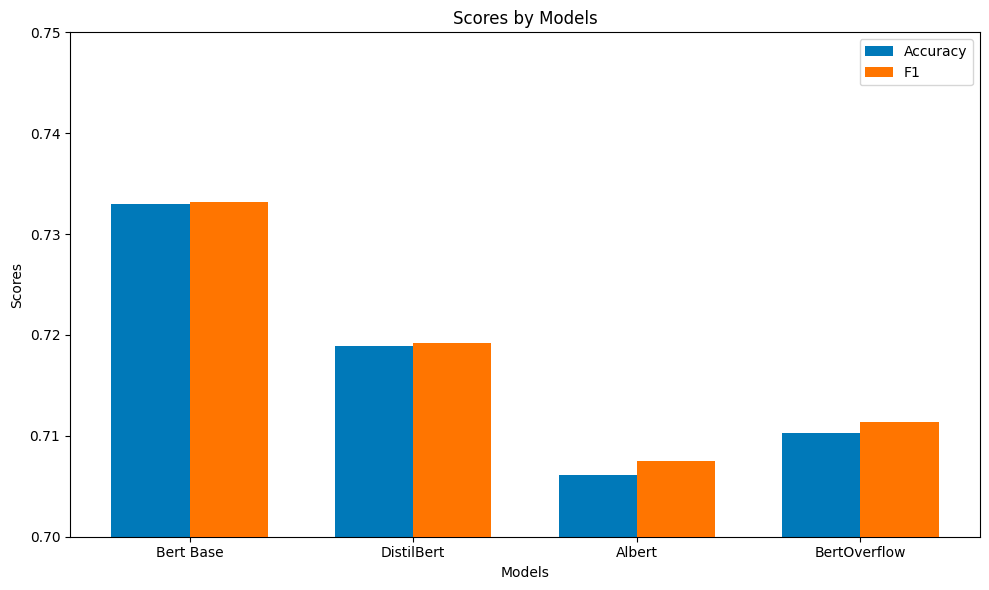
\includegraphics[width=\textwidth]{./figures/model-accuracy}
        \caption{Bar chart showing the accuracy of the models}
        \label{fig:accuracy}
    \end{figure}



    The Bert-base-uncased model performed the best, followed by the Distilbert model.
    Distilbert was faster to train than the Bert-base-uncased model, taking 240 minutes to train for 25 epochs, compared to 380 to train for 20 epochs.
    This would mean that the Distilbert model would be more cost effective to train, as it would take less time to train. However it is less accurate, so a trade-off would need to be made between accuracy and cost.
    TODO compare prediction times

    The Albert model performed the worst, with an accuracy of 0.7061, and a F1 score of 0.7075. Although pe

    \chapter{Finalised Model and Results }
    \label{ch:results}

    This chapter discusses the final model, and the results of testing the model on the test set.
    It also discusses the results of testing the model on a different unrelated project, to see how well the model generalises to unseen data.
    Finally I perform an ablation study to see how well the model performs without the paraphrased data, custom loss function and data preprocessing.


    \section{Results}
    The final model was trained on the entire dataset, and then tested on the test set.
    This test set was not used in the training of the model but is from the same projects, and therefore is a good representation of how the model will perform on unseen but related data.
    I then tested it on a set of tickets from a different project, to see how well it generalised to unseen data that is more likely to be different from the training data.

    A seperate test set was used rather than using the validation set. This is because the validation set was used to compare the models, and therefore the model may have been overfit to the validation set.
    The results are shown in table .

    The results show that the model performs better on the classes for small and large, and worse on the medium class.
    This is likely due to the fact that the medium class is the most ambiguous, and therefore the hardest to classify, even for a human.
    The confusion matrix in TODO:  shows...


\begin{table}
\centering
\begin{tblr}{
  cells = {c},
  cell{1}{2} = {c=4}{},
  cell{2}{1} = {r=4}{},
  vlines,
  hline{1-2,6} = {-}{},
  hline{3-5} = {2-5}{},
}

                                            & Predicted Labels &     &     &     \\
\begin{sideways}Actual Labels\end{sideways} &                  & 0   & 1   & 2   \\
                                            & 0                & 442 & 242 & 32  \\
                                            & 1                & 207 & 753 & 192 \\
                                            & 2                & 34  & 218 & 541
\end{tblr}
\caption{Confusion Matrix}
\end{table}
    The model was then tested on a different project, and the results are shown in table TODO: \par
    The results show that the model does not perform well on a different project, and therefore the model may not generalise well to unseen data.
    This is likely due to the fact that the model has been trained on a specific set of projects, and the project tested is for a plaform team, that mostly creates automations and cloud resources which is very different to the automotive projects in the training data .

    In order to compare the model to human estimation accuracy, I used the set of tickets that had been estimated with a specific time and that had an actual time documented to compare to.
    I then placed the estimaed and actual time into the same catagories as for the model, small, medium and large.
    From this i was able to calculate the accuracy of the model, and the results show that the human accuracy is 0.77.
    This is 3-4\% higher than the model, however the model is able to estimate the tickets much faster than a human, and therefore is more efficient.
    Furthermore, as the model is trained on tickets throughout the entire history of the project, the model is able to estimate tickets that are similar to ones that have been estimated before, and therefore the model is able to learn from the history of the project, rather than just the tickets that have been estimated or worked on by the person, or people, estimating the tickets.

    \section{Ablation Study}
    In order to see how much the paraphrased data, custom loss function and data preprocessing helped the model, I removed each in turn, testing the model on the test set after each change and also the unseen data from a seperate project.
    I trained the model on the original dataset without adding the paraphrased data. The aim of this is to see if the model performs better with the paraphrased data or if the paraphrasing is too different from the original data and it doesnt help, or if the data is too similar and overfits.
    The results show that the model performs better with the paraphrased data, and therefore the paraphrased data will be used in the final model.
    I then trained the model on the original dataset without using Guassian Distribution as the label for cross entropy loss.  This is to see if the custom loss function helps the model to learn the sequential nature of the classes.
    The results show that the model performs better with the custom loss function, and therefore the custom loss function will be used in the final model.
    However it is only a small improvement, and therefore the model may be able to be simplified by using the standard cross entropy loss function.
    I then trained the model on the original dataset without using the data cleaner. This is to see if the data cleaner helps the model to learn the context of the tickets, or if context is lost in the cleaning process.
    The results show that the model actually performed almost the same without the data. Although the datacleaner removes syntax and allows more of the text of the description to be used, it may be that the model is able to learn from the syntax in relation to the context of the ticket.
    Further experiments could be done to see if the data cleaner is actually needed, or if the model can learn the context of the ticket without it given more fine tuning and potentially more data.
    The results of these tests are shown in table TODO: \par


    % Test with a validation set and then a test set from a different project and also unseen tickets from the same project




    % Add a table of results
    % Test final model on unseen projects data and compare to previous models



    \chapter{Model as a Service}
    \label{ch:model-as-a-service}
    \subsection[Proposed User Experience]{Proposed User Experience}


    \chapter{Conclusion and further work}
    \label{ch:conclusion}

\printbibliography

\end{document}
